\documentclass{article}
\usepackage[margin=1in]{geometry}
\usepackage{ragged2e}
\usepackage{enumerate}
\usepackage{graphicx}
\usepackage{rotating}
\usepackage{float}


\usepackage{listings}
\usepackage{color}

\definecolor{dkgreen}{rgb}{0,0.6,0}
\definecolor{gray}{rgb}{0.5,0.5,0.5}
\definecolor{mauve}{rgb}{0.58,0,0.82}
\definecolor{darkblue}{rgb}{0.0,0.0,0.6}
\definecolor{cyan}{rgb}{0.0,0.6,0.6}

 \lstset{frame=tb,
  language=Java,
  breaklines=true,
  showstringspaces=false,
  columns=flexible,
  numbers=none,
  commentstyle=\color{dkgreen},
  stringstyle=\color{mauve},
  tabsize=3
}
\lstdefinelanguage{XML}
{
  morestring=[b]",
  morestring=[s]{>}{<},
  morecomment=[s]{<?}{?>},
  stringstyle=\color{black},
  identifierstyle=\color{darkblue},
  keywordstyle=\color{cyan},
  morekeywords={xmlns,version,type,ma-id}% list your attributes here
}


\begin{document}

%%%%%%%%%%%%%%%%%%%%%%%%%%%%%%%%%%%%%%%%%%%%%%%%%%%%%%%%%%%%%%%%%%%%%%%%%%%%%%%%%%%%%%%%%%%%%%%%
% DISCLAIMER COVER SHEET
%%%%%%%%%%%%%%%%%%%%%%%%%%%%%%%%%%%%%%%%%%%%%%%%%%%%%%%%%%%%%%%%%%%%%%%%%%%%%%%%%%%%%%%%%%%%%%%%

\begin{titlepage}
	\noindent Project 2 \hfill CS170: Introduction to Artificial Intelligence \newline \newline
	Audrey Der \hfill Dr. Eamonn Keogh \newline
	861221280 \newline
	ader003@ucr.edu \newline
	15-12-17 \newline \newline \newline
	In completing this assignment I consulted:
	\begin{itemize}
		\item The slides from lecture.
        \item Python 2.7.14, 3.5, and 3.6 Documentation. This is the URL to the Table of Contents of 2.7.14:  https://docs.python.org/2/contents.html
        \item The NumPy 1.13 Manual: https://docs.scipy.org/doc/numpy-1.13.0/index.html
	\end{itemize}
	All important code is original. Unimportant subroutines that are not completely original are\ldots
	\begin{itemize}
		\item \textbf{numpy} library, to load the data in, normalize it, and other data-related manipulations and calculations
        \item \textbf{math} library, for calculations
        \item \textbf{random}, for testing
        \item \textbf{time}, for report related purposes
        \end{itemize}
        \end{titlepage}

%%%%%%%%%%%%%%%%%%%%%%%%%%%%%%%%%%%%%%%%%%%%%%%%%%%%%%%%%%%%%%%%%%%%%%%%%%%%%%%%%%%%%%%%%%%%%%%%
% WRITE UP FUN
%%%%%%%%%%%%%%%%%%%%%%%%%%%%%%%%%%%%%%%%%%%%%%%%%%%%%%%%%%%%%%%%%%%%%%%%%%%%%%%%%%%%%%%%%%%%%%%%

\title{CS170 Project 2 Write Up: Feature Selection with Nearest Neighbor}
\author{Audrey Der, 861221280}
\date{\today}
\maketitle

\section{Introduction}
This is write up details the second project in Dr. Eamonn Keogh's course on Artifical
Intelligence (Fall 2017). The project explores the success of the nearest neighbor
algorithm under different feature selection searches. Nearest neighbors
is sensitive to irrelevant features, making fruitful to search for
the best set of features when applying the algorithm.

\subsection{Project-Specific Details}
The project calls for the following search algorithms to be implemented: forward selection, backward
elimination, and a custom algorithm from the student. The custom algorithm is
designed to be faster, more accurate, or both, than forward selection and
backward elimination. \\

For the purposes of the assignment, each student was assigned a unique pair of data
sets to consider. One small, with 10 features, and the other large, with 50
features. The files I was to consider were \textbf{CS170Smalltestdata\_\_32.txt}
and \textbf{CS170BIGtestdata\_\_71.txt}. \\

This report includes a full copy of the implementation and a sample output using
my custom algorithm on data set with 50 features and two possible classifications.

\section{Algorithms}
\subsection{Forward Selection}
On a high level, forward selection considers all subsets of features in the
data's given features by adding features to an empty set. It returns the set of
most accurate features.

\subsection{Backward Elimination}
Backward elimination also considers all subsets of features, but begins with the
entire set of given features, and removes features from the set. It returns the
set of most accurate features.

\subsection{Forward's Propinqua: Faster Forward Selection}
\textbf{Propinqua}: (\textit{Latin}) feminine singular form of 'propinquo',
meaning ``next, near'' 

Forward selection returns the best set of features by keeping track of the
current best set it as it considers each subset of features. However, in
principle, nearest neighbors and a set of only the best features $S$ will perform
better than nearest neighbors on $S$ with any \textit{additional} features. \\ 

Consider a set of current best features $S_1$ with an accuracy of $a_1$. Suppose
accuracy begins to decline after the addition of a feature $f_i$ to $S_1$ (call
this set of features $S_{f_i}$). Any feature set $S$ where $S_{f_i}$ is a
subset of $S$ will never yield an accuracy greater than $a_1$. It can be concluded
that exploring any set $S$ containing $S_{f_i}$ is likely to be unfruitful.
This, in theory should significantly decrease the time the algorithm spends
searching for the most accurate set of features. \\

\subsection{Caveats and Deductions: Local Maxima and Why Greedy is Conditionally Acceptable}

My custom algorithm implements that principle in three lines of python. However,
Forward's Propinqua is quite greedy. It is extremely sensitive to local maxima; it breaks should it find
one. Because of the risk of returning a local maxima, some algorithms may opt to
continue searching $n$ many further feature additions in the case a local maxima
was hit (and the global maxima is yet to come), but Forward's Propinqua does not. \\

To reiterate: Forward's Propinqua will miss the true best set after returning a
local maxima. Despite this incredible blind spot in the algorithm, Forward's
Propinqua still works just about as well as forward selection with my specifically assigned datasets. Perhaps this is why:
\begin{itemize}
\item As can be seen in the results (detailed later in this report), Forward
  Selection was more accurate than backward elimination on both datasets. Forward selection performing better indicates that the features in the
  datasets were more independent than correlated.
\item Because the features were more independent than related, \textbf{the risk
    of not exploring a feature subset that produces a pair or set of features that work
    very well together is significantly reduced}.
\item So conversely, on a dataset with highly related features, Forward's
  Propinqua will perform terribly.
\end{itemize}

\subsection{Proof of Reduced Cycle Time}

Figure 1 (pg.3) is a chart of Cycle Times on the large and small datasets between forward
selection and Propinqua.

\section{Results}

My implementation of the assignment's results in comparison to Professor Keogh's
key:
\begin{itemize}
  
\item The Small Dataset, best features:
  \begin{itemize}
  \item \textbf{Forward Selection:} [9, 6, 1], Reported accuracy: 95.960%
  \item \textbf{Backward Elimination:} [1, 8, 9, 10], Reported accuracy: 90.909%
  \item \textbf{Propinqua:} [9, 6, 1], Reported accuracy: 95.960%
  \item \textbf{Professor Keogh's Key:} [9, 3, 6] with 3 being a weak feature
  \end{itemize}
   With respect to Professor Keogh's Key, Forward Selection was better
   than Backward Elimination, yielding two correct features and one spurious
   feature. It missed the weak good feature. Figure 2 (pg.4) was based on
   \textbf{CS170Smalltestdata\_\_32.txt}. 
  
\item The Large Dataset, best features:
  \begin{itemize}
  \item \textbf{Forward Selection:} [24, 19, 25], Reported accuracy: 97.980%
  \item \textbf{Backward Elimination:} [1, 3, 5, 6, 7, 8, 10, 12, 13, 14, 15,
    16, 17, 20, 21, 22, 24, 25, 26, 27, 29, 30, 32, 34, 35, 36, 38, 40, 42, 43,
    44, 45, 46, 47, 48, 49, 50], Reported accuracy: 86.869%
  \item \textbf{Propinqua:} [24, 19, 25], Reported accuracy: 97.980%
  \item \textbf{Professor Keogh's Key:} [24, 34, 19]
    \end{itemize}
\end{itemize}
  With respect to Professor Keogh's Key, Forward Selection was better than
  Backward Elimination, yielding two correct features and one spurious feature.
  It missed one feature. Figures 3-4 (pgs.5-6) was based on
  \textbf{CS170BIGtestdata\_\_71.txt}. 

\section{Conclusion}
Considering the results and performances of forward selection and backward
elimination, it can be said that:
\begin{itemize}
\item Depending on how correlated the features are, either forward selection
  or backward elimination will perform better than the other. Forward
  selection is more accurate when features are highly independent, and
  backward elimination is more accurate when features are highly related.
  Regarding the given datasets \textbf{CS170BIGtestdata\_\_71.txt} and
  \textbf{CS170Smalltestdata\_\_32.txt}, forward selection performed better.
\item Returned feature sets may vary based on the implementation of a given
  algorithm, due to the randomness of each. However, if the search algorithms
  are implemented correctly, some strong features should still be detected.
\item Forward's Propinqua exploits the nature of feature sets with independent
  features. In feature sets with independent features, finding the best feature
  set can be made faster whilst still using the same intuition behind forward
  selection by stopping the search with a subset of features that produces an
  accuracy lower than the current best global accuracy. While Forward's
  Propinqua remains sensitive to local maxima, the liklihood of running into
  local maxima is not as high when used on feature sets with independent features.
 
\end{itemize}

\section{Figures: Charts and Graphs}

  \begin{figure}[!h]
  \centering
  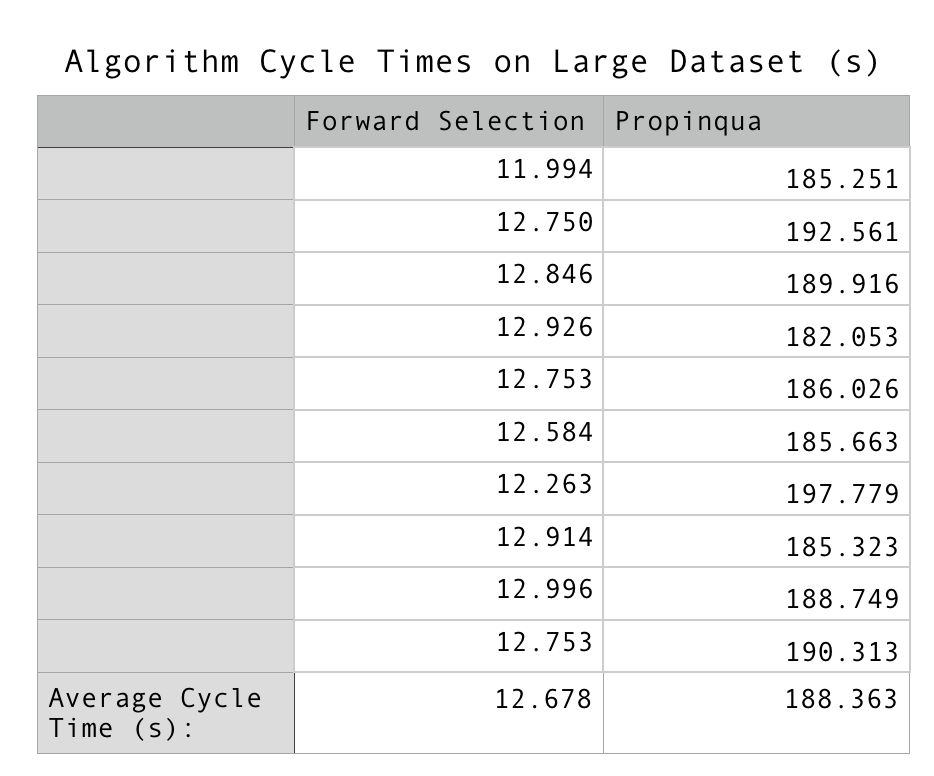
\includegraphics[width=8cm,keepaspectratio]{AvgCycleTime.png}
  \caption{Average Cycle Times for Forward Selection and Propinqua. DISCLAIMER: A more accurate estimate of the true cycle time requires many, many more
recordings of elapsed time. However, due to time constraints, the above can be
held as a loose approximation.}
\end{figure}
\clearpage

   \begin{figure}[!h]
  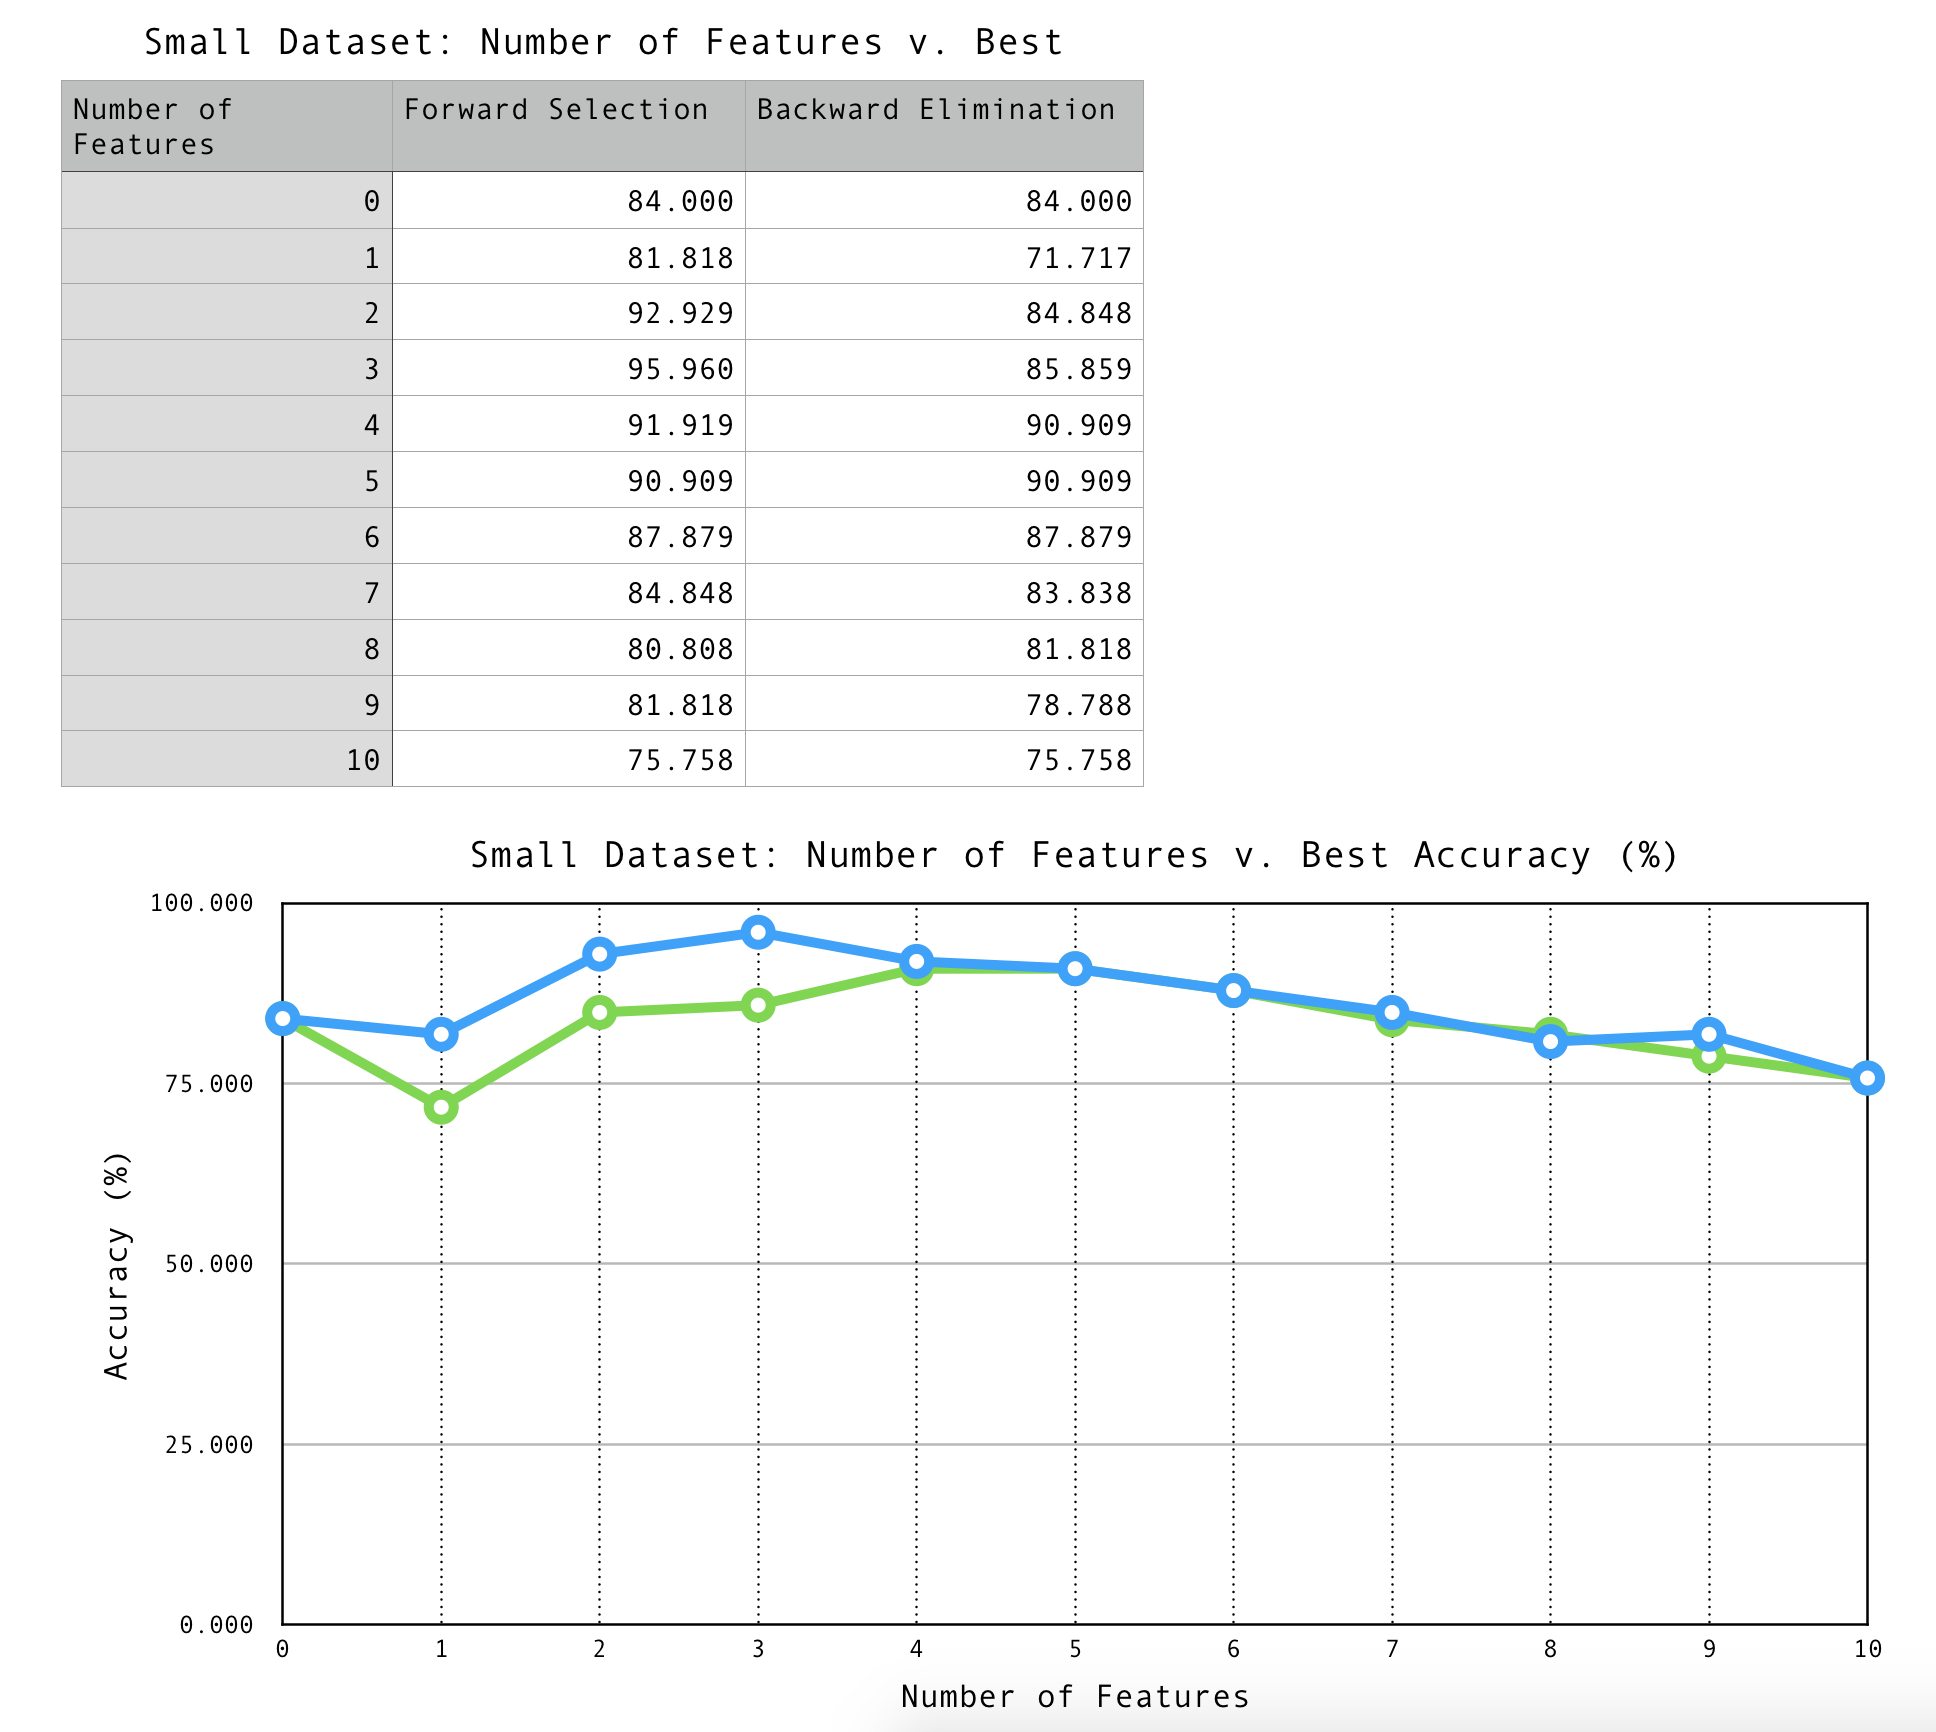
\includegraphics[width=\textwidth,height=\textheight,keepaspectratio]{SmallDataSetGraph.png}
  \caption{Small Dataset and Graph}
\end{figure}
\clearpage

\begin{sidewaysfigure}
  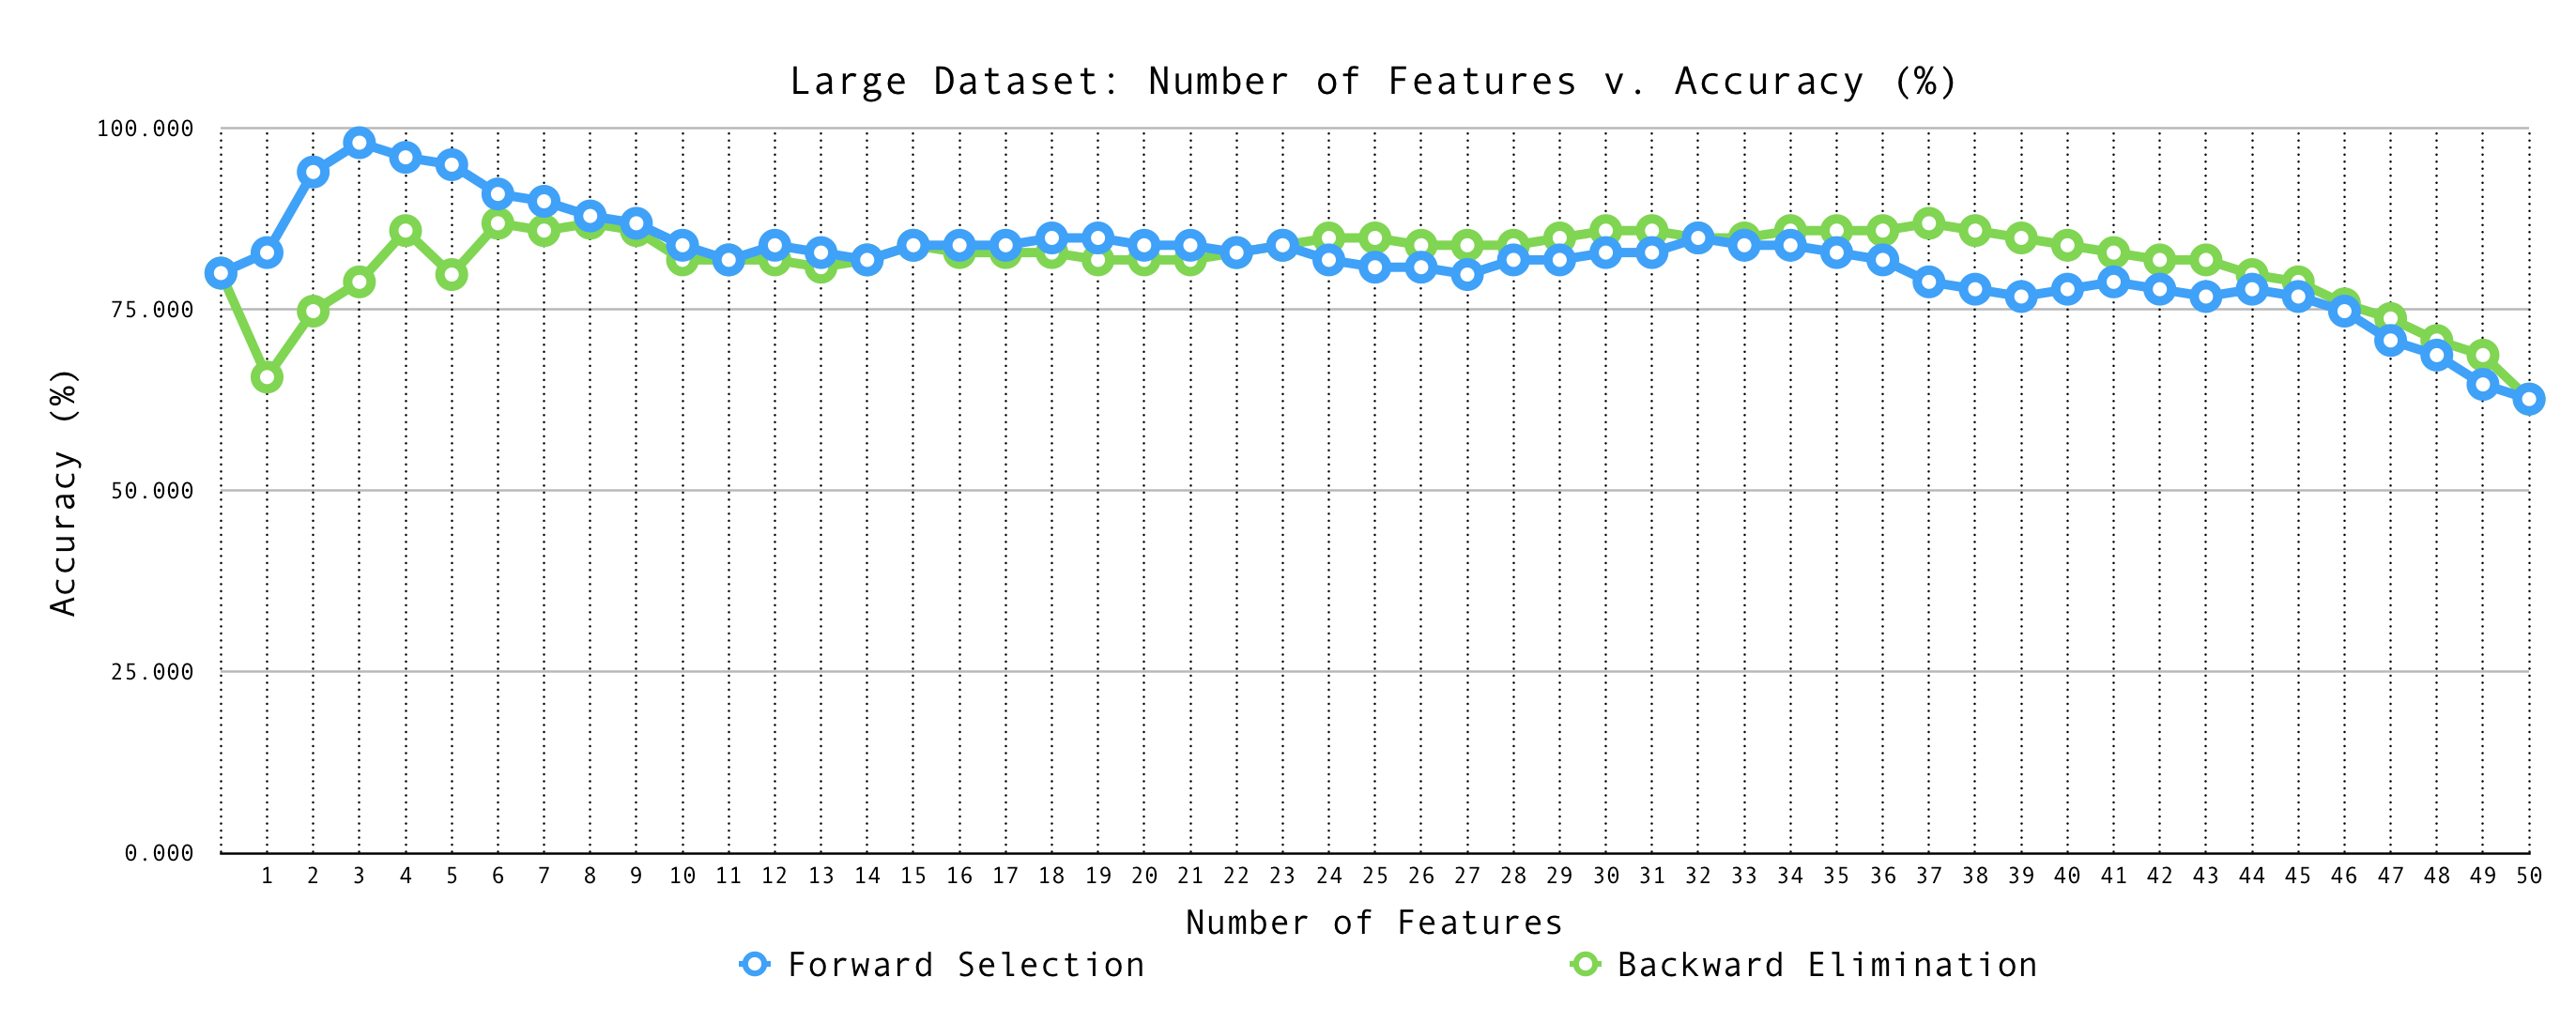
\includegraphics[width=\textwidth,height=\textheight,keepaspectratio]{LargeTestDataGraph.png}
  \caption{Graph based on Large Dataset}
\end{sidewaysfigure}
\clearpage

\begin{sidewaysfigure}
  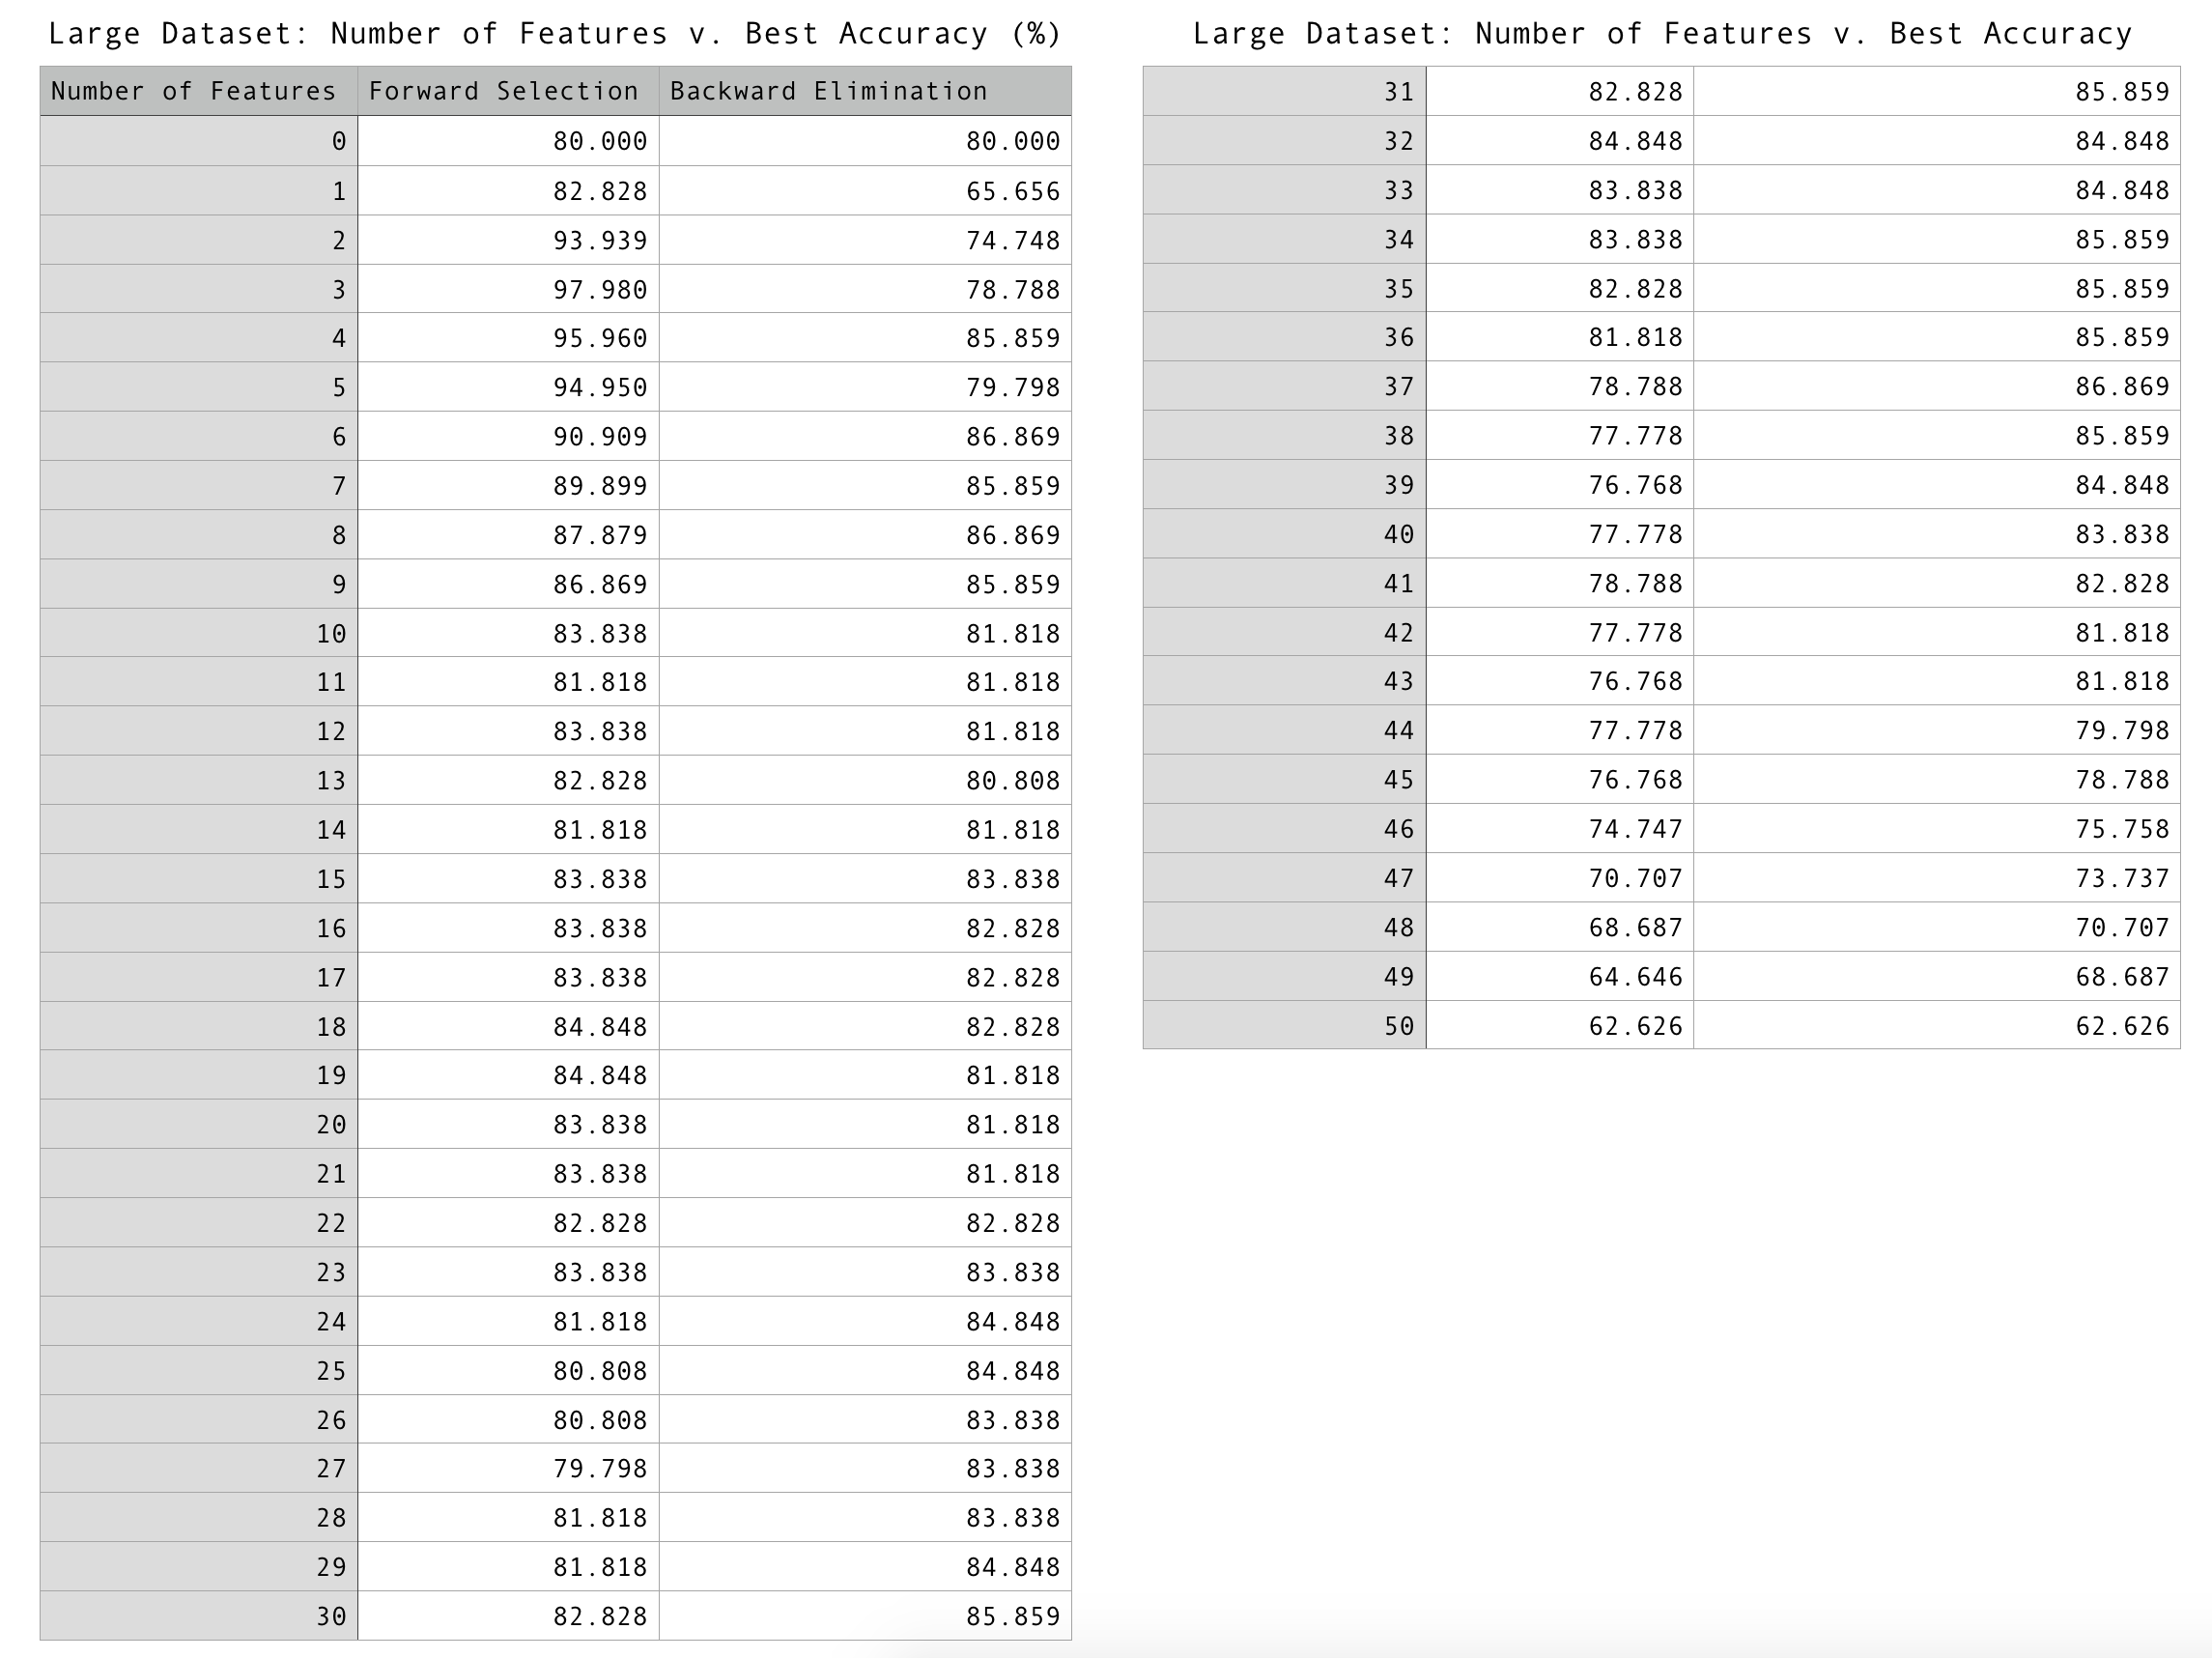
\includegraphics[width=\textwidth,height=\textheight,keepaspectratio]{LargeTestData.png}  
  \caption{Large Dataset Data}
\end{sidewaysfigure}
\clearpage

%%%%%%%%%%%%%%%%%%%%%%%%%%%%%%%%%%%%%%%%%%%%%%%%%%%%%%%%%%%%%%%%%%%%%%%%%%%%%%%%%%%%%%%%%%%%%%%%
%TRACEBACK TIME
%%%%%%%%%%%%%%%%%%%%%%%%%%%%%%%%%%%%%%%%%%%%%%%%%%%%%%%%%%%%%%%%%%%%%%%%%%%%%%%%%%%%%%%%%%%%%%%%
\section{Traceback and Code}
Here is a traceback of forward selection using the data from
\textbf{CS170Smalltestdata\_\_32.txt}:
\begin{lstlisting}[captionpos=b, caption=Traceback, label=listing:sparql_getallindividuals,
   basicstyle=\ttfamily]

Select the algorithm you wish to use: 
1. Forward Selection
2. Backwards Elimination
3. Propinqua Algorithm
1
Please hold while data is normalized.
... Done!
--Considering adding feature  1
--Considering adding feature  2
--Considering adding feature  3
--Considering adding feature  4
--Considering adding feature  5
--Considering adding feature  6
--Considering adding feature  7
--Considering adding feature  8
--Considering adding feature  9
--Considering adding feature  10
On level  1  feature  9  was added to the current set
With  1  features, the accuracy is:  81.81818181818183 %
--Considering adding feature  1
--Considering adding feature  2
--Considering adding feature  3
--Considering adding feature  4
--Considering adding feature  5
--Considering adding feature  6
--Considering adding feature  7
--Considering adding feature  8
--Considering adding feature  10
On level  2  feature  6  was added to the current set
With  2  features, the accuracy is:  92.92929292929293 %
--Considering adding feature  1
--Considering adding feature  2
--Considering adding feature  3
--Considering adding feature  4
--Considering adding feature  5
--Considering adding feature  7
--Considering adding feature  8
--Considering adding feature  10
On level  3  feature  1  was added to the current set
With  3  features, the accuracy is:  95.95959595959596 %
--Considering adding feature  2
--Considering adding feature  3
--Considering adding feature  4
--Considering adding feature  5
--Considering adding feature  7
--Considering adding feature  8
--Considering adding feature  10
On level  4  feature  5  was added to the current set
With  4  features, the accuracy is:  91.91919191919192 %
--Considering adding feature  2
--Considering adding feature  3
--Considering adding feature  4
--Considering adding feature  7
--Considering adding feature  8
--Considering adding feature  10
On level  5  feature  8  was added to the current set
With  5  features, the accuracy is:  90.9090909090909 %
--Considering adding feature  2
--Considering adding feature  3
--Considering adding feature  4
--Considering adding feature  7
--Considering adding feature  10
On level  6  feature  7  was added to the current set
With  6  features, the accuracy is:  87.87878787878788 %
--Considering adding feature  2
--Considering adding feature  3
--Considering adding feature  4
--Considering adding feature  10
On level  7  feature  3  was added to the current set
With  7  features, the accuracy is:  84.84848484848484 %
--Considering adding feature  2
--Considering adding feature  4
--Considering adding feature  10
On level  8  feature  4  was added to the current set
With  8  features, the accuracy is:  80.8080808080808 %
--Considering adding feature  2
--Considering adding feature  10
On level  9  feature  2  was added to the current set
With  9  features, the accuracy is:  81.81818181818183 %
--Considering adding feature  10
On level  10  feature  10  was added to the current set
With  10  features, the accuracy is:  75.75757575757575 %
Set of features used:  [9, 6, 1] at accuracy:  95.95959595959596 
 Elapsed time:  4.512928009033203
  
  \end{lstlisting}


%%%%%%%%%%%%%%%%%%%%%%%%%%%%%%%%%%%%%%%%%%%%%%%%%%%%%%%%%%%%%%%%%%%%%%%%%%%%%%%%%%%%%%%%%%%%%%%%
%CODE SHENANIGANS
%%%%%%%%%%%%%%%%%%%%%%%%%%%%%%%%%%%%%%%%%%%%%%%%%%%%%%%%%%%%%%%%%%%%%%%%%%%%%%%%%%%%%%%%%%%%%%%%
The full implementation is as follows:
\begin{lstlisting}[captionpos=b, caption=Impementation, label=listing:sparql_getallindividuals,
   basicstyle=\ttfamily]

  import numpy as np
import math
import random
import time


def select_algorithm():
    algorithm = input("Select the algorithm you wish to use: " + '\n' +
                      "1. Forward Selection" + '\n' +
                      "2. Backwards Elimination" + '\n' +
                      "3. Propinqua Algorithm" + '\n'
                      )  # "Propinquus" is latin for "near/neighboring"

    # print("Please hold while the data is normalized.")
    # normalize_data()
    return algorithm


def normalize_data(data):
    print("Please hold while data is normalized.")
    data = (data - np.mean(data)) / np.std(data)
    print("... Done!")
    return data


def forward_selection(data):
    curr_set_of_features = []
    global_best_acc = 0.0 # global best accuracy
    overall_best_feat_set = [] # global best feature
    start_time = time.time()
    for i in range(1, len(data[0])): # acts as a multiplier; how many times to run the inner loop
        feat_to_add = 0
        local_best_acc = 0.0 # best recorded accuracy for local levels
        for k in range(1, len(data[0])): # runs through the features and calculates accuracy based on the current set with the new addition
            if k not in curr_set_of_features:
                print("--Considering adding feature ", k)
                acc = find_accuracy(curr_set_of_features, data, k, 1)
                if acc > local_best_acc:
                    local_best_acc = acc
                    feat_to_add = k
        curr_set_of_features.append(feat_to_add) # appends feature selected by inner for loop
        print("On level ", i, " feature ", feat_to_add, " was added to the current set")
        print("With ", len(curr_set_of_features), " features, the accuracy is: ", local_best_acc * 100, "%")
        if local_best_acc >= global_best_acc: # check for decrease in accuracy
            global_best_acc = local_best_acc
            overall_best_feat_set = list(curr_set_of_features)
    end_time = time.time()
    print("Set of features used: ", overall_best_feat_set, "at accuracy: ", global_best_acc * 100, '\n', "Elapsed time: ", end_time - start_time)
    return


def backwards_elimination(data):
    global_best_acc = 0.0 # global best accuracy
    overall_best_feat_set = []
    curr_set_of_features = [i for i in range(1, len(data[0]))]
    start_time = time.time()
    for i in range(1, len(data[0]) - 1):
        feat_to_pop = 0
        local_best_acc = 0.0 # best recorded accuracy for local levels
        for k in range(1, len(data[0]) - 1):
            if k in curr_set_of_features:
                print("--Considering adding feature ", k)
                acc = find_accuracy(curr_set_of_features, data, k, 2)
                if acc > local_best_acc:
                    local_best_acc = acc
                    feat_to_pop = k
        if feat_to_pop in curr_set_of_features: 
            curr_set_of_features.remove(feat_to_pop) # removes feature selected by inner for loop
            print("On level ", i, " feature ", feat_to_pop, " was removed from the current set")
            print("With ", len(curr_set_of_features), " features, the accuracy is: ", local_best_acc * 100, "%")
        if local_best_acc >= global_best_acc: # check for decrease in accuracy
            global_best_acc = local_best_acc
            overall_best_feat_set = list(curr_set_of_features)
    end_time = time.time()
    print("Set of features used: ", overall_best_feat_set, "At accuracy: ", global_best_acc * 100, '\n', "Elapsed time: ", end_time - start_time)
    return

def propinqua(data): #forward selection with pruning
    print("You have selected the custom Propinqua Algorithm. Please note that only the best feature tests will be printed.")
    curr_set_of_features = []
    global_best_acc = 0.0 # global best accuracy
    overall_best_feat_set = [] # global best feature
    start_time = time.time()
    for i in range(1, len(data[0])): # acts as a multiplier; how many times to run the inner loop
        feat_to_add = 0
        local_best_acc = 0.0 # best recorded accuracy for local levels
        for k in range(1, len(data[0])): # runs through the features and calculates accuracy based on the current set with the new addition
            if k not in curr_set_of_features:
                acc = find_accuracy(curr_set_of_features, data, k, 1)
                if acc > local_best_acc:
                    local_best_acc = acc
                    feat_to_add = k
        if local_best_acc <= global_best_acc:
            if k == len(data[0]) - 1: # if the addition of any feature not yet included results in a decrease in accuracy, the best set has been found; break out of loop
                break
        if local_best_acc > global_best_acc: # check for decrease in accuracy
            curr_set_of_features.append(feat_to_add) # appends feature selected by inner for loop
            global_best_acc = local_best_acc
            overall_best_feat_set = list(curr_set_of_features)
        print("Set of current features (algorithm still in progress): ", curr_set_of_features)
        print("Accuracy at current level: ", local_best_acc * 100, "%")
    end_time = time.time()
    print("Set of features used: ", overall_best_feat_set, "At accuracy: ", global_best_acc * 100, "%", '\n', "Elapsed time: ", end_time - start_time)
    return


def read_in_data(filename):
    return np.loadtxt(filename)


def find_accuracy(set_of_features, data, test_feature, algorithm):
    test_feat_set = list(set_of_features)
    if algorithm == 1: #forward selection; Custom 
        test_feat_set.append(test_feature)
    if algorithm == 2: #backwards elimination
        test_feat_set.remove(test_feature)
    num_correct_classifications = 0
    local_shortest_distance = math.inf
    result = 0 # will be either 1 or 2
    for i in data:
        local_shortest_distance = math.inf
        for h in data:
            if not np.array_equal(h, i): #checks if h and i are not the same row
                distance = 0
                for j in test_feat_set:
                    distance += pow((i[j] - h[j]), 2.0) # n-space Euclidean distance formula
                if math.sqrt(distance) < local_shortest_distance:
                    local_shortest_distance = math.sqrt(distance)
                    result = h[0] # the result "guessed" by the algorithm
        if result == i[0]:
            num_correct_classifications += 1
    return num_correct_classifications / (len(data) - 1)


def main():
    filename = input("Type in the name of the file to test: ")
    algorithm = select_algorithm()
    if algorithm == "1":
        forward_selection(normalize_data(read_in_data(filename)))
    if algorithm == "2":
       backwards_elimination(normalize_data(read_in_data(filename)))
    if algorithm == "3":
       propinqua(normalize_data(read_in_data(filename)))
    return

if __name__ == '__main__':
    main()


\end{lstlisting}

\end{document}